\section{Experiments and Analysis}
We evaluated the Universal Transformer on a range of algorithmic and language understanding tasks, as well as on machine translation. We describe these tasks and datasets in more detail in Appendix~\ref{app:desc-tasks}. All code and datasets reproducing these results will be released as open source.

\subsection{bAbI Question-Answering}
The bAbi question answering dataset~\citep{weston2015towards} consists of 20 different synthetic tasks\footnote{\url{https://research.fb.com/downloads/babi}}. The aim is that each task tests a unique aspect of language understanding and reasoning, including the ability of: reasoning from supporting facts in a story, answering true/false type questions, counting, understanding negation and indefinite knowledge, understanding coreferences, time reasoning, positional and size reasoning, path-finding, and understanding motivations (to see examples for each of these tasks, please refer to Table 1 in \citep{weston2015towards}).

There are two versions of the dataset, one with 1k training examples and the other with 10k examples. It is important for a model to be data-efficient to achieve good results using only the 1k training examples. Moreover, the original idea is that a single model should be evaluated across all the tasks (not tuning per task), which is the \emph{train joint} setup in Tables~\ref{tab:babi-results} and ~\ref{tbl:babi_details}.

A standard Transformer does not achieve good results on this task\footnote{We experimented with different hyper-parameters and different network sizes, but it always overfits.}. However, we have designed a model based on the Universal Transformer which achieves state-of-the-art results on this task.

To encode the input, similar to~\cite{henaff2016tracking}, we first encode each fact in the story by applying a learned multiplicative positional mask to each word's embedding, and summing up all embeddings.
We embed the question in the same way, and then feed the (Universal) Transformer with these embeddings of the facts and questions. 

As originally proposed, models can either be trained on each task separately (``train single'') or jointly on all tasks (``train joint''). Table~\ref{tab:babi-results} summarizes our results. We conducted 10 runs with different initializations and picked the best model based on performance on the validation set, similar to previous work. Both the UT and UT with dynamic halting achieve state-of-the-art results on all tasks in terms of average error and number of failed tasks\footnote{Defined as $> 5\%$ error.}, in both the 10K and 1K training regime. Tables~\ref{tbl:babi_details} presents the results of best and average results of 10 runs breakdown by task.

\begin{table}[t!]
\centering
\begin{adjustbox}{max width=\textwidth}
\begin{tabular}{lllll}
& & & & \\ \toprule
\multirow{2}{*}{ \bf Model } & \multicolumn{2}{c}{ \bf 10K examples } & \multicolumn{2}{c}{ \bf 1K examples } \\ \cmidrule{2-5}
& train single & train joint & train single & train joint \\ \midrule
\multicolumn{5}{c}{\bf Previous best results:} \\ \midrule
QRNet~\citep{seo2016query} & 0.3 (0/20) & - & - & - \\
Sparse DNC~\citep{rae2016scaling} & - & 2.9 (1/20) & - & - \\
GA+MAGE~\cite{dhingra2017linguistic} & - & - & 8.7 (5/20) & - \\
MemN2N~\cite{sukhbaatar2015} & - & - & -  & 12.4 (11/20) \\\midrule
\multicolumn{5}{c}{\bf Our Results:} \\ \midrule
Transformer~\citep{transformer} & 15.2 (10/20) & 22.1 (12/20) & 21.8 (5/20) & 26.8 (14/20) \\
Universal Transformer (this work) & 0.23 (0/20) & 0.47 (0/20) & 5.31 (5/20) & 8.50 (8/20) \\
UT w/ dynamic halting (this work) & {\bf 0.21 (0/20)} & {\bf 0.29 (0/20)} & {\bf 4.55 (3/20)} & {\bf 7.78 (5/20)} \\ \bottomrule
\end{tabular}
\end{adjustbox}
\caption{Average error and number of failed tasks ($> 5\%$ error) out of 20 (in parentheses; lower is better in both cases) on the bAbI dataset under the different training/evaluation setups. We indicate state-of-the-art where available for each, or `-' otherwise.}
\label{tab:babi-results}
\end{table}
\begin{table}[t!]
\centering
\caption{Detailed results on the bAbI question answering tasks.}
\label{tbl:babi_details}
\begin{subtable}{0.6\textwidth}
\centering
\begin{adjustbox}{max width=\textwidth}
\begin{tabular}{lcccc}
\toprule
\multicolumn{5}{c}{Best seed run for each task (out of 10 runs) } \\ \midrule
\multirow{2}{*}{ Task id } & \multicolumn{2}{c}{ 10K } & \multicolumn{2}{c}{ 1K } \\  \cmidrule{2-5}
& train single & train joint & train single & train joint \\ \midrule
1 & 0.0 & 0.0 & 0.0 & 0.0 \\
2 & 0.0 & 0.0 & 0.0 & 0.5 \\
3 & 0.4 & 1.2 & 3.7 & 5.4 \\
4 & 0.0 & 0.0 & 0.0 & 0.0 \\
5 & 0.0 & 0.0 & 0.0 & 0.5 \\
6 & 0.0 & 0.0 & 0.0 & 0.5 \\
7 & 0.0 & 0.0 & 0.0 & 3.2 \\
8 & 0.0 & 0.0 & 0.0 & 1.6 \\
9 & 0.0 & 0.0 & 0.0 & 0.2 \\
10 & 0.0 & 0.0 & 0.0 & 0.4 \\
11 & 0.0 & 0.0 & 0.0 & 0.1 \\
12 & 0.0 & 0.0 & 0.0 & 0.0 \\
13 & 0.0 & 0.0 & 0.0 & 0.6 \\
14 & 0.0 & 0.0 & 0.0 & 3.8 \\
15 & 0.0 & 0.0 & 0.0 & 5.9 \\
16 & 0.4 & 1.2 & 5.8 & 15.4 \\
17 & 0.6 & 0.2 & 32.0 & 42.9 \\
18 & 0.0 & 0.0 & 0.0 & 4.1 \\
19 & 2.8 & 3.1 & 47.1 & 68.2 \\
20 & 0.0 & 0.0 & 2.4 & 2.4 \\ \midrule
avg err & 0.21 & 0.29 & 4.55 & 7.78 \\ \midrule
failed & 0 & 0 & 3 & 5 \\
\bottomrule
\end{tabular}
\end{adjustbox}
\end{subtable}
\\
\vspace{10pt}
\begin{subtable}{0.6\textwidth}
\centering
\begin{adjustbox}{max width=\textwidth}
\begin{tabular}{lcccc}
\toprule
\multicolumn{5}{c}{Average (\rpm var) over all seeds (for 10 runs)} \\ \midrule
\multirow{2}{*}{ Task id } & \multicolumn{2}{c}{ 10K } & \multicolumn{2}{c}{ 1K } \\  \cmidrule{2-5}
& train single & train joint & train single & train joint \\ \midrule
1 & 0.0 \rpm 0.0 & 0.0 \rpm 0.0 & 0.2 \rpm 0.3 & 0.1 \rpm 0.2 \\ 
2 & 0.2 \rpm 0.4 & 1.7 \rpm 2.6 & 3.2 \rpm 4.1 & 4.3 \rpm 11.6 \\ 
3 & 1.8 \rpm 1.8 & 4.6 \rpm 7.3 & 9.1 \rpm 12.7 & 14.3 \rpm 18.1 \\ 
4 & 0.1 \rpm 0.1 & 0.2 \rpm 0.1 & 0.3 \rpm 0.3 & 0.4 \rpm 0.6 \\ 
5 & 0.2 \rpm 0.3 & 0.8 \rpm 0.5 & 1.1 \rpm 1.3 & 4.3 \rpm 5.6 \\ 
6 & 0.1 \rpm 0.2 & 0.1 \rpm 0.2 & 1.2 \rpm 2.1 & 0.8 \rpm 0.4 \\ 
7 & 0.3 \rpm 0.5 & 1.1 \rpm 1.5 & 0.0 \rpm 0.0 & 4.1 \rpm 2.9 \\ 
8 & 0.3 \rpm 0.2 & 0.5 \rpm 1.1 & 0.1 \rpm 0.2 & 3.9 \rpm 4.2 \\ 
9 & 0.0 \rpm 0.0 & 0.0 \rpm 0.0 & 0.1 \rpm 0.1 & 0.3 \rpm 0.3 \\ 
10 & 0.1 \rpm 0.2 & 0.5 \rpm 0.4 & 0.7 \rpm 0.8 & 1.3 \rpm 1.6 \\ 
11 & 0.0 \rpm 0.0 & 0.1 \rpm 0.1 & 0.4 \rpm 0.8 & 0.3 \rpm 0.9 \\ 
12 & 0.2 \rpm 0.1 & 0.4 \rpm 0.4 & 0.6 \rpm 0.9 & 0.3 \rpm 0.4 \\ 
13 & 0.2 \rpm 0.5 & 0.3 \rpm 0.4 & 0.8 \rpm 0.9 & 1.1 \rpm 0.9 \\ 
14 & 1.8 \rpm 2.6 & 1.3 \rpm 1.6 & 0.1 \rpm 0.2 & 4.7 \rpm 5.2 \\ 
15 & 2.1 \rpm 3.4 & 1.6 \rpm 2.8 & 0.3 \rpm 0.5 & 10.3 \rpm 8.6 \\ 
16 & 1.9 \rpm 2.2 & 0.9 \rpm 1.3 & 9.1 \rpm 8.1 & 34.1 \rpm 22.8 \\ 
17 & 1.6 \rpm 0.8 & 1.4 \rpm 3.4 & 43.7 \rpm 18.6 & 51.1 \rpm 12.9 \\ 
18 & 0.3 \rpm 0.4 & 0.7 \rpm 1.4 & 2.3 \rpm 3.6 & 12.8 \rpm 9.0 \\ 
19 & 3.4 \rpm 4.0 & 6.1 \rpm 7.3 & 50.2 \rpm 8.4 & 73.1 \rpm 23.9 \\ 
20 & 0.0 \rpm 0.0 & 0.0 \rpm 0.0 & 3.2 \rpm 2.5 & 2.6 \rpm 2.8 \\ \midrule
avg & 0.73 \rpm 0.89 & 1.12 \rpm 1.62 & 6.34 \rpm 3.32 & 11.21 \rpm 6.65 \\ 
\bottomrule
\end{tabular}
\end{adjustbox}
\end{subtable}
\end{table}
\afterpage{\clearpage}


To understand the working of the model better, we analyzed both the attention distributions and the average ACT ponder times for this task. First, we observe that the attention distributions start out very uniform, but get progressively sharper in later steps around the correct supporting facts that are required to answer each question, which is indeed very similar to how humans would solve the task. 
%
Second, with dynamic halting we observe that the average ponder time (i.e.\ depth of the per-symbol recurrent processing chain) over all positions in all samples in the test data for tasks requiring three supporting facts is higher ($3.8 \rpm 2.2$) than for tasks requiring only two ($3.1 \rpm 1.1$), which is in turn higher than for tasks requiring only one supporting fact ($2.3 \rpm 0.8$). This indicates that the model adjusts the number of processing steps with the number of supporting facts required to answer the questions. 

\begin{figure}[t]
 \centering
 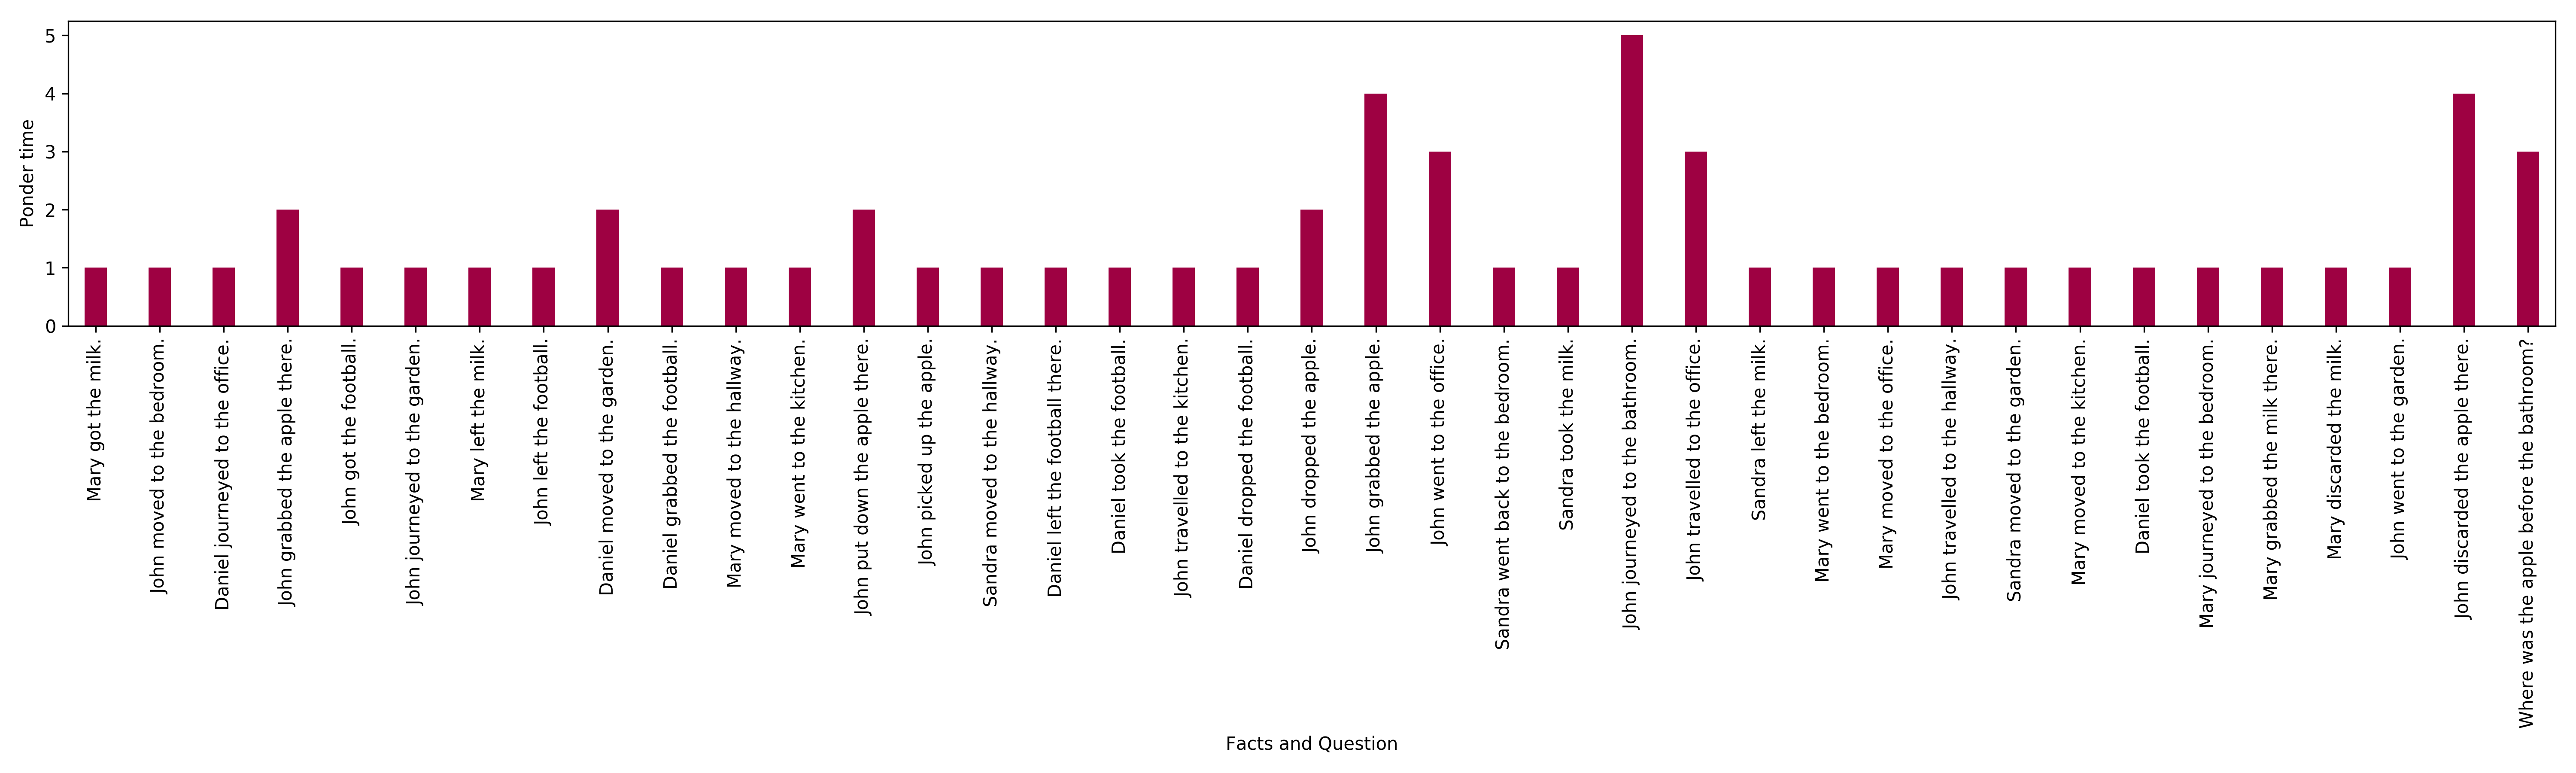
\includegraphics[width=\textwidth]{04-part-03/chapter-06/figs_and_tables/fig_task3_example_ponder.png}
 \caption{Ponder time of UT with dynamic halting for encoding facts in a story and question in a bAbI task requiring three supporting facts.}
 \label{fig:act_ponder}
\end{figure}
Finally, we observe that the histogram of ponder times at different positions is more uniform in tasks requiring only one supporting fact compared to two and three, and likewise for tasks requiring two compared to three.  Especially for tasks requiring three supporting facts, many positions halt at step 1 or 2 already and only a few get transformed for more steps (see for example Figure~\ref{fig:act_ponder}). This is particularly interesting as the length of stories is indeed much higher in this setting, with more irrelevant facts which the model seems to successfully learn to ignore in this way.

Similar to dynamic memory networks~\citep{kumar2016ask}, there is an iterative attention process in UTs that allows the model to condition its attention over memory on the result of previous iterations. 
%
Figures~\ref{fig:ex1}, \ref{fig:ex2}, \ref{fig:ex3}, and \ref{fig:ex4} present visualizations of the attention distributions on bAbI tasks for some examples from Task 1, 2, and 3. The visualization of attention weights is over different time steps based on different heads over all the facts in the story and a question. Different color bars on the left side indicate attention weights based on different heads (4 heads in total).

\begin{figure}[!ht]
\begin{minipage}{\textwidth}
\fontsize{8}{8}\fontfamily{pcr}\selectfont
\begin{tabular}{l l}
\textbf{An example from tasks 1}: & \textbf{(requiring one supportive fact to solve)}\\
\\
\textbf{Story}: & \\
& John travelled to the hallway. \\
& Mary journeyed to the bathroom. \\
& Daniel went back to the bathroom. \\
& John moved to the bedroom \\
\\
\textbf{Question}: & \\
& Where is Mary? \\
\textbf{Model's output}: & \\
& bathroom
\end{tabular}
\end{minipage}
\\ \vfill
\vspace{20pt} % maximize space between the minipages
\begin{minipage}{\textwidth}
    \centering
    \begin{subfigure}[t]{\textwidth}
        \centering
        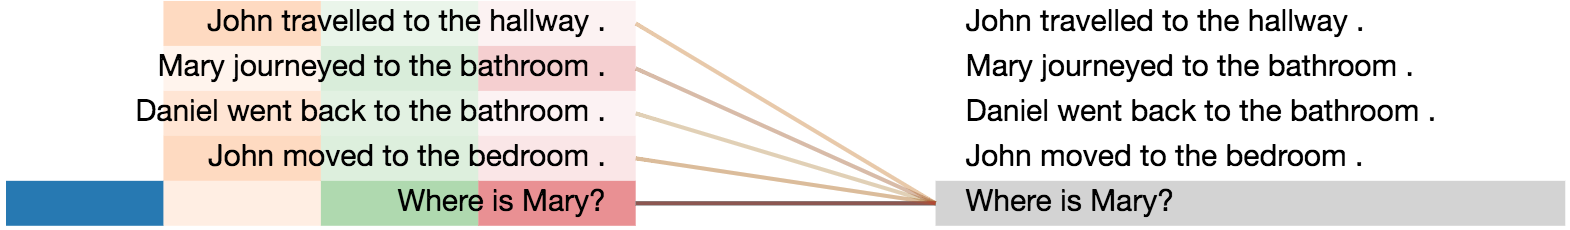
\includegraphics[height=0.8in]{04-part-03/chapter-06/figs_and_tables/figs_attention_babi/e1-step1.png}
        \caption{Step 1}
    \end{subfigure}%
    \hfill \hfill
    \begin{subfigure}[t]{\textwidth}
        \centering
        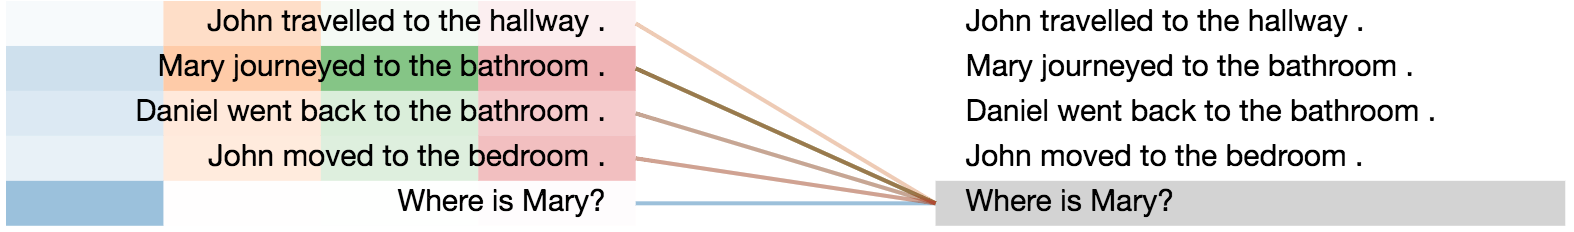
\includegraphics[height=0.8in]{04-part-03/chapter-06/figs_and_tables/figs_attention_babi/e1-step2}
        \caption{Step 2}
    \end{subfigure}
    \hfill \hfill
    \begin{subfigure}[t]{\textwidth}
        \centering
        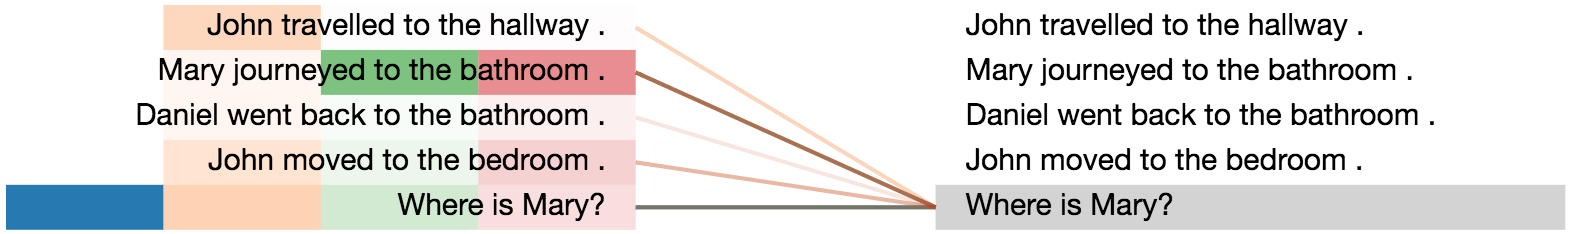
\includegraphics[height=0.8in]{04-part-03/chapter-06/figs_and_tables/figs_attention_babi/e1-step3}
        \caption{Step 3}
    \end{subfigure}
    \hfill \hfill 
    \begin{subfigure}[t]{\textwidth}
        \centering
        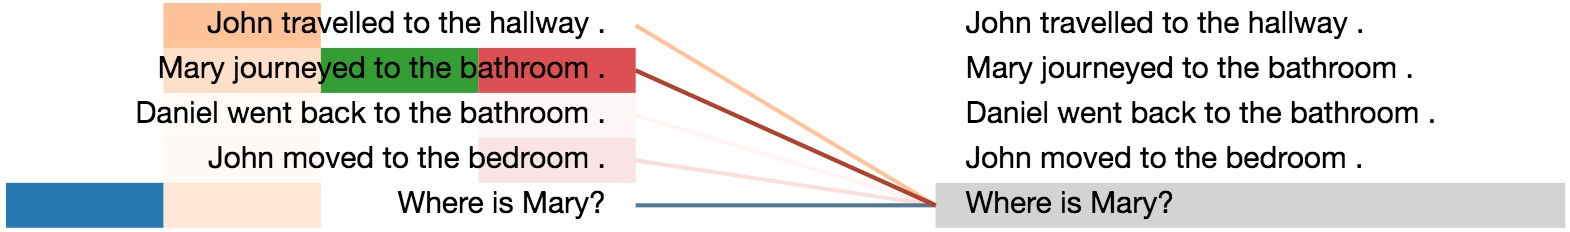
\includegraphics[height=0.8in]{04-part-03/chapter-06/figs_and_tables/figs_attention_babi/e1-step4}
        \caption{Step 4}
    \end{subfigure}
\end{minipage}
    \caption{\label{fig:ex1}Visualization of the attention distributions, when encoding the question: \emph{``Where is Mary?''}.}
\end{figure}
\afterpage{\clearpage}




\begin{figure}[!h]
\begin{minipage}{\textwidth}
\fontsize{8}{8}\fontfamily{pcr}\selectfont
\begin{tabular}{l l}
\textbf{An example from tasks 2}: & \textbf{(requiring two supportive facts to solve)}\\
\\
\textbf{Story}: & \\
& Sandra journeyed to the hallway. \\
& Mary went to the bathroom. \\
& Mary took the apple there. \\
& Mary dropped the apple. \\
\\
\textbf{Question}: & \\
& Where is the apple? \\
\textbf{Model's output}: & \\
& bathroom
\end{tabular}
\end{minipage}
\\  \vfill
\vspace{20pt} % maximize space between the minipages
\begin{minipage}{\textwidth}
    \centering
    \begin{subfigure}[t]{\textwidth}
        \centering
        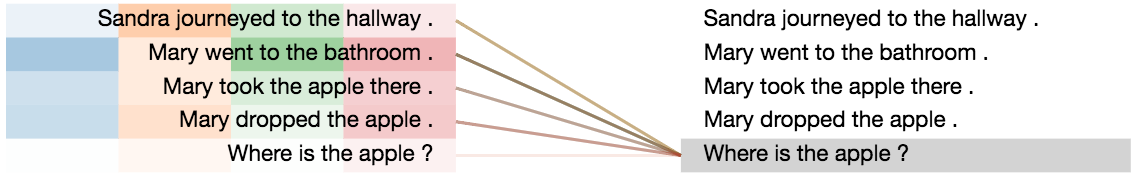
\includegraphics[height=0.8in]{04-part-03/chapter-06/figs_and_tables/figs_attention_babi/e2-step1}
        \caption{Step 1}
    \end{subfigure}%
    \hfill \hfill
    \begin{subfigure}[t]{\textwidth}
        \centering
        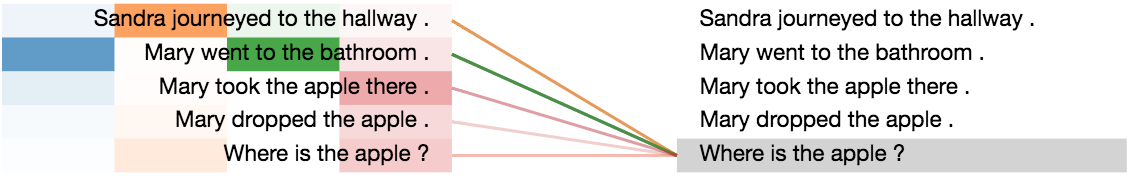
\includegraphics[height=0.8in]{04-part-03/chapter-06/figs_and_tables/figs_attention_babi/e2-step2}
        \caption{Step 2}
    \end{subfigure}
    \hfill \hfill
    \begin{subfigure}[t]{\textwidth}
        \centering
        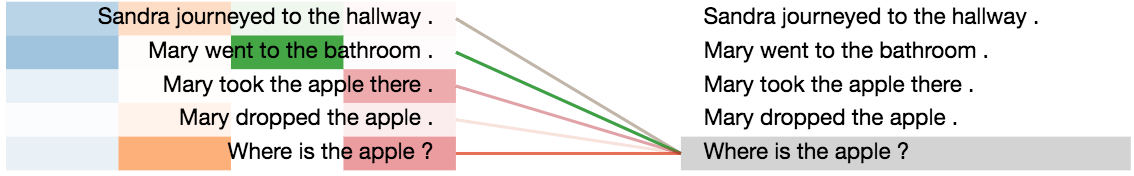
\includegraphics[height=0.8in]{04-part-03/chapter-06/figs_and_tables/figs_attention_babi/e2-step3}
        \caption{Step 3}
    \end{subfigure}
    \hfill \hfill 
    \begin{subfigure}[t]{\textwidth}
        \centering
        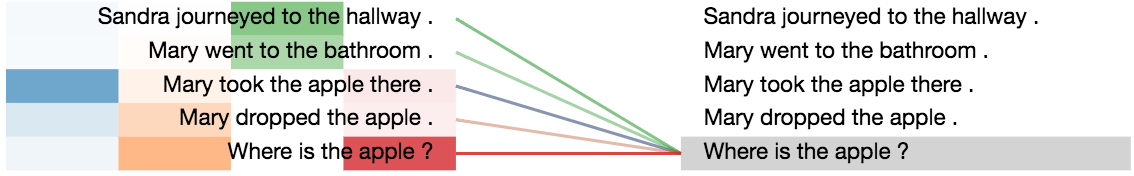
\includegraphics[height=0.8in]{04-part-03/chapter-06/figs_and_tables/figs_attention_babi/e2-step4}
        \caption{Step 4}
    \end{subfigure}
    \end{minipage}
    \caption{\label{fig:ex2}Visualization of the attention distributions, when encoding the question: \emph{``Where is the apple?''}.}
\end{figure}

\afterpage{\clearpage}

\begin{figure}[!h]
\begin{minipage}{\textwidth}
\fontsize{8}{8}\fontfamily{pcr}\selectfont
\begin{tabular}{l l}
\textbf{An example from tasks 2}: & \textbf{(requiring two supportive facts to solve)}\\
\\
\textbf{Story}: & \\
& John went to the hallway. \\
& John went back to the bathroom. \\
& John grabbed the milk there. \\
& Sandra went back to the office. \\
& Sandra journeyed to the kitchen. \\
& Sandra got the apple there. \\
& Sandra dropped the apple there. \\
& John dropped the milk. \\
\\
\textbf{Question}: & \\
& Where is the milk? \\
\textbf{Model's output}: & \\
& bathroom
\end{tabular}
\end{minipage}
\\ \vfill
\vspace{20pt} % maximize space between the minipages
\begin{minipage}{\textwidth}
    \centering
    \begin{subfigure}[t]{\textwidth}
        \centering
        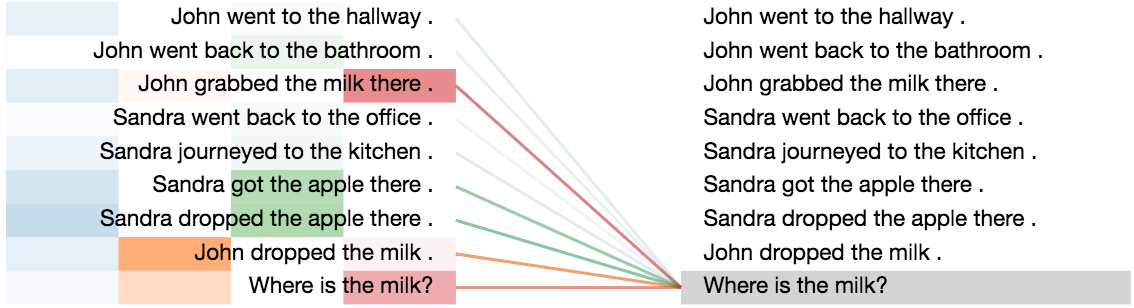
\includegraphics[height=1.3in]{04-part-03/chapter-06/figs_and_tables/figs_attention_babi/e3-step1}
        \caption{Step 1}
    \end{subfigure}%
    \hfill \hfill
    \begin{subfigure}[t]{\textwidth}
        \centering
        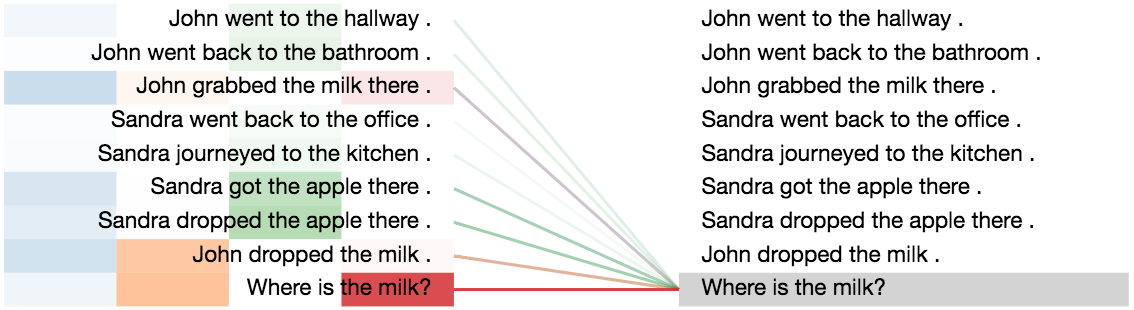
\includegraphics[height=1.3in]{04-part-03/chapter-06/figs_and_tables/figs_attention_babi/e3-step2}
        \caption{Step 2}
    \end{subfigure}
    \hfill \hfill
    \begin{subfigure}[t]{\textwidth}
        \centering
        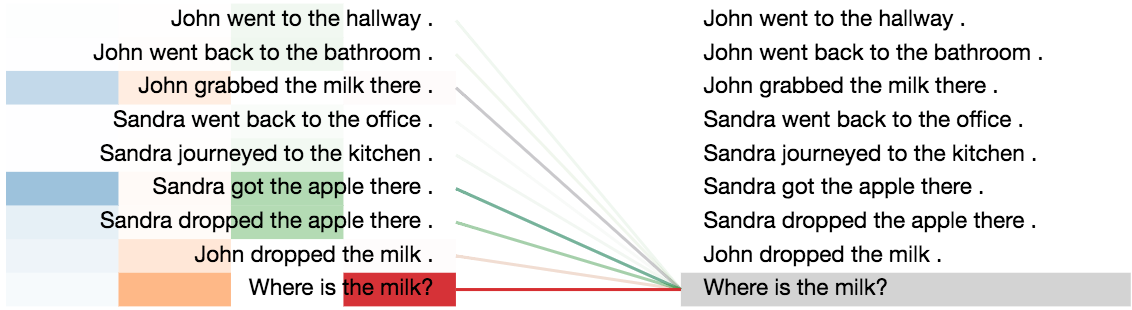
\includegraphics[height=1.3in]{04-part-03/chapter-06/figs_and_tables/figs_attention_babi/e3-step3}
        \caption{Step 3}
    \end{subfigure}
    \hfill \hfill 
    \begin{subfigure}[t]{\textwidth}
        \centering
        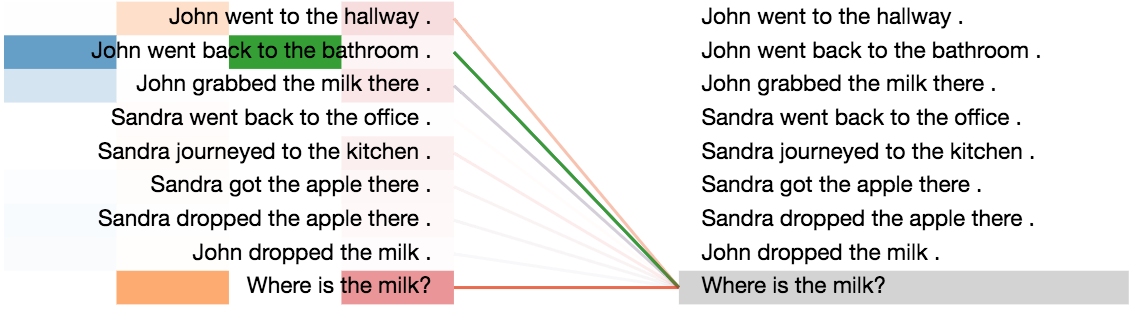
\includegraphics[height=1.3in]{04-part-03/chapter-06/figs_and_tables/figs_attention_babi/e3-step4}
        \caption{Step 4}
    \end{subfigure}
    \end{minipage}
    \caption{\label{fig:ex3}Visualization of the attention distributions, when encoding the question: \emph{``Where is the milk?''}.}
\end{figure}

\afterpage{\clearpage}

\begin{figure}[!h]
\begin{minipage}{\textwidth}
\fontsize{8}{8}\fontfamily{pcr}\selectfont
\begin{tabular}{l l}
\textbf{An example from tasks 3}: & \textbf{(requiring three supportive facts to solve)}\\
\\

\textbf{Story}: & \\
Mary got the milk. \\
& John moved to the bedroom. \\
& Daniel journeyed to the office. \\
& John grabbed the apple there. \\
& John got the football. \\
& John journeyed to the garden. \\
& Mary left the milk. \\
& John left the football. \\
& Daniel moved to the garden. \\
& Daniel grabbed the football. \\
& Mary moved to the hallway. \\
& Mary went to the kitchen. \\
& John put down the apple there. \\
& John picked up the apple. \\
& Sandra moved to the hallway. \\
& Daniel left the football there. \\
& Daniel took the football. \\
& John travelled to the kitchen. \\
& Daniel dropped the football. \\
& John dropped the apple. \\
& John grabbed the apple. \\
& John went to the office. \\
& Sandra went back to the bedroom. \\
& Sandra took the milk. \\
& John journeyed to the bathroom. \\
& John travelled to the office. \\
& Sandra left the milk. \\
& Mary went to the bedroom. \\
& Mary moved to the office. \\
& John travelled to the hallway. \\
& Sandra moved to the garden. \\
& Mary moved to the kitchen. \\
& Daniel took the football. \\
& Mary journeyed to the bedroom. \\
& Mary grabbed the milk there. \\
& Mary discarded the milk. \\
& John went to the garden. \\
& John discarded the apple there. \\
\\
\textbf{Question}: & \\
& Where was the apple before the bathroom? \\
\textbf{Model's output}: & \\
& office
\end{tabular}
\end{minipage}
\end{figure}
\begin{figure}[h!]\ContinuedFloat
\begin{minipage}{\textwidth}
    \centering
    \begin{subfigure}[t]{\textwidth}
        \centering
        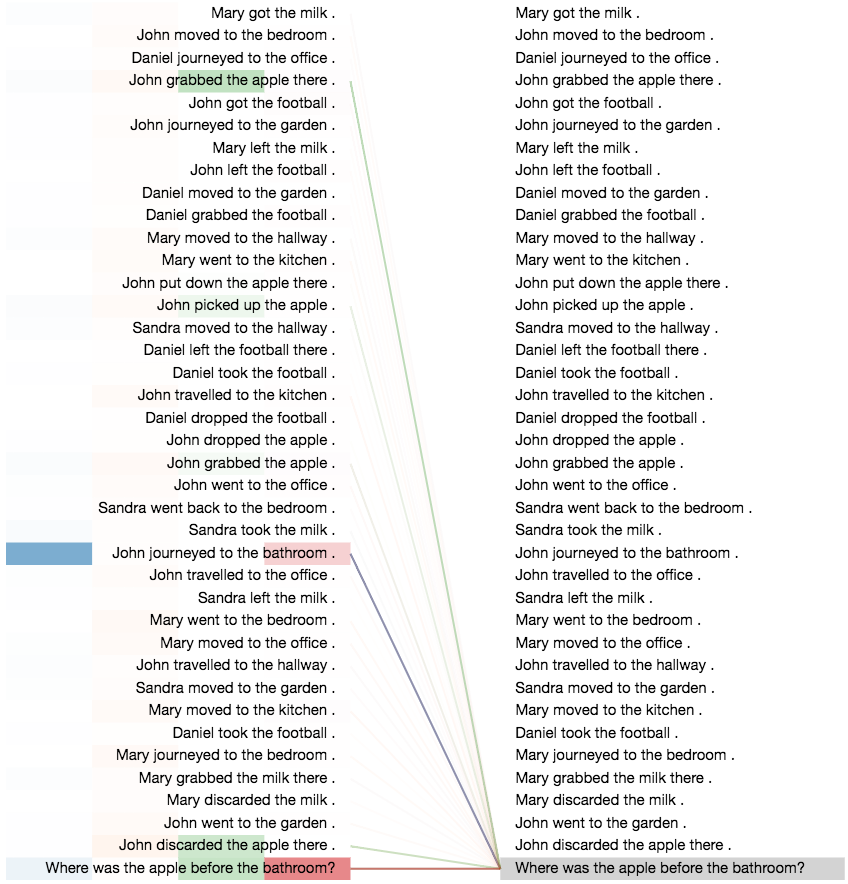
\includegraphics[height=4.2in]{04-part-03/chapter-06/figs_and_tables/figs_attention_babi/e4-step1}
        \caption{Step 1}
    \end{subfigure}%
    \hfill \hfill
    \begin{subfigure}[t]{\textwidth}
        \centering
        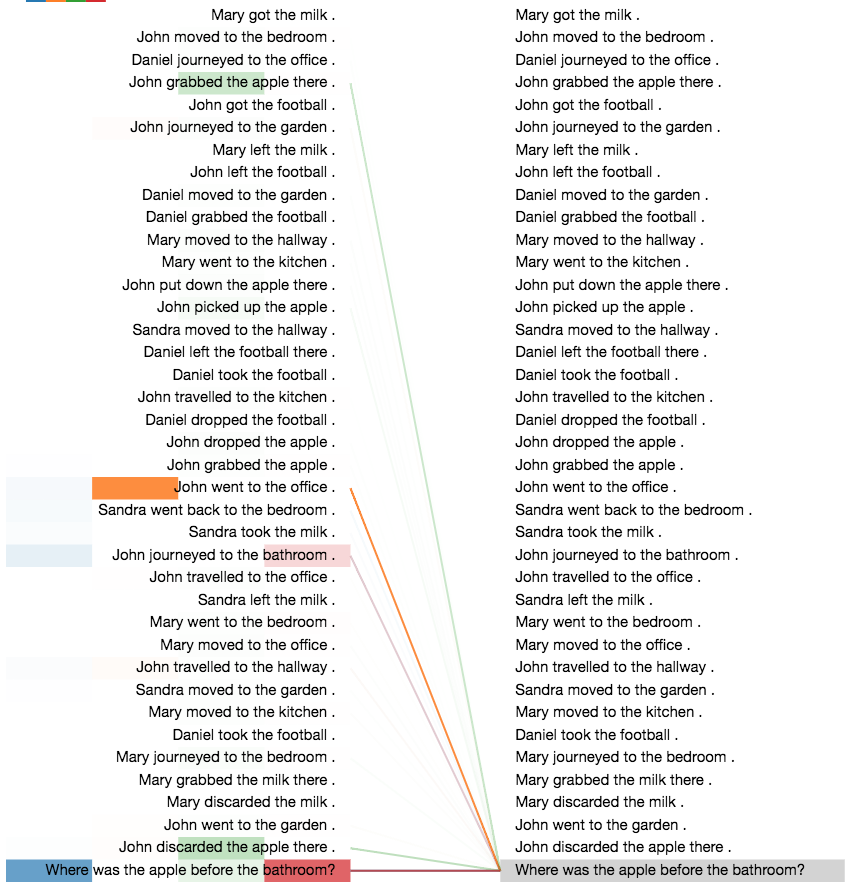
\includegraphics[height=4.2in, trim={0 0 0 0.1cm},clip]{04-part-03/chapter-06/figs_and_tables/figs_attention_babi/e4-step2}
        \caption{Step 2}
    \end{subfigure}
\end{minipage}
\end{figure}
\begin{figure}[h!]\ContinuedFloat
\begin{minipage}{\textwidth}\ContinuedFloat
    \begin{subfigure}[t]{\textwidth}
        \centering
        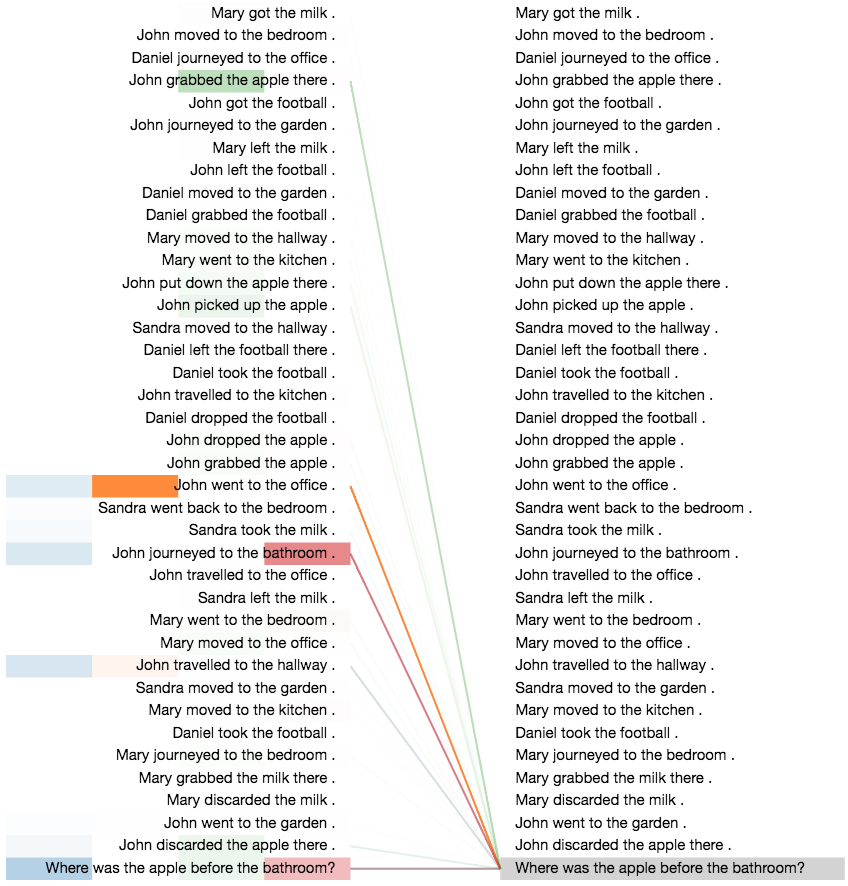
\includegraphics[height=4.2in]{04-part-03/chapter-06/figs_and_tables/figs_attention_babi/e4-step3}
        \caption{Step 3}
    \end{subfigure}
    \hfill \hfill 
    \begin{subfigure}[t]{\textwidth}
        \centering
        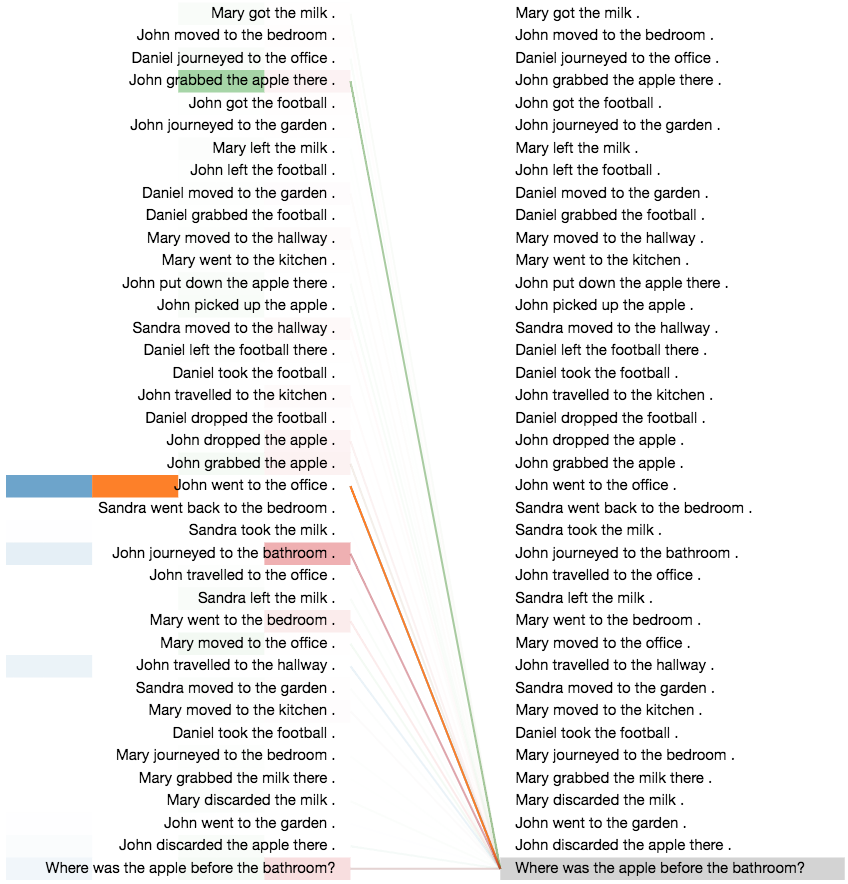
\includegraphics[height=4.2in]{04-part-03/chapter-06/figs_and_tables/figs_attention_babi/e4-step4}
        \caption{Step 4}
    \end{subfigure}
    \caption{\label{fig:ex4}Visualization of the attention distributions, when encoding the question: \emph{``Where was the apple before the bathroom?''}.}
\end{minipage}
\end{figure}

The above examples illustrate that there is a notion of temporal states in UT, where the model updates its states (memory) in each step based on the output of previous steps, and this chain of updates can also be viewed as steps in a multi-hop reasoning process.
